\documentclass{article}
\usepackage{graphicx}
\usepackage{amsmath} % define math env \align \endalign
\usepackage{amssymb}% contains the definition of \triangleq,\mathcal
\usepackage{bm}
\usepackage{mathtools}
\DeclarePairedDelimiter\abs{\lvert}{\rvert}
\DeclarePairedDelimiter\norm{\lVert}{\rVert}
\def\E{\mathbb{E}}
\def\Y{\mathcal{Y}}
\def\T{\mathrm{T}}
\DeclareMathOperator\diag{diag}
\DeclareMathOperator\artanh{artanh}
% decrease the margin as Professor Huang said
% \usepackage[a4paper,margin=2cm]{geometry}
\begin{document}
\begin{figure}[!ht]
\centering
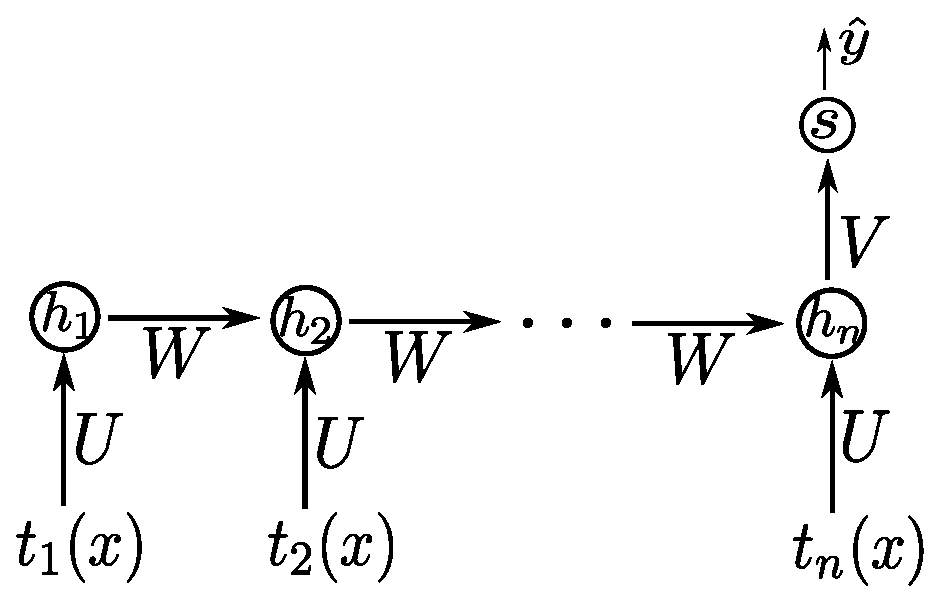
\includegraphics[width=6cm]{rnn.eps}
\end{figure}
% recurrent nerual network
Consider a simple rnn(shown in the figure above), we approximate the distribution $P_{Y|X}$ by the softmax output of rnn: $\tilde{P}_{Y|X}(k|x) \triangleq \hat{y}_k(x)$. The parameters (mainly matrix $U,W$) in the different layers of network are shared and are optimized by network training process. We consider special case when $X,Y$ are weakly correlated and the problem is to find the structure of optimal $U$ and $W$ given $V$ and $P_{Y|X}$.

First, we formulate above problem mathmetically. The loss function to minimize has the form (cross entropy loss) 
\begin{equation}\label{eq:cel}
L=-\E_{P_{X,Y}}\log \tilde{P}_{Y|X}
\end{equation}
(in practial calculation $P_{X,Y}$ is replaced by empirical distribution $\hat{P}_{X,Y}$ which is learned from sample). For rnn network, we have
\begin{subequations}
\begin{align}
\label{eq:h_i} h_i & =  \tanh (W h_{i-1} + U t_i)\\
\label{eq:last_layer} \hat{y}_k & = \frac{\exp(v^T_k h_n+b_k)}{\sum_k \exp(v_k h_n+b_k)},k=1,2,\dots,|\Y|
\end{align}
\end{subequations}
%where $V=[v^\T_1,v^\T_2,\dots,v^\T_{|\Y|}],v_k $ is row vector.
Let $h_i(x,j)$ denotes the $j$\hspace{-0.4pt}-th element of the vector $h_i(x)$, then from \eqref{eq:h_i} we have
\begin{equation}\label{eq:act_item}
h_i(x,j)= \tanh (w_j h_{i-1}(x)+u_j t_i(x,j))
\end{equation}
where $w_j,u_j$ are row vectors respectively.

Suppose $\epsilon$ is  \textbf{small}, and we have the following two assumptions:
\begin{enumerate}
\item $\abs{w_j h_{i-1}(x)}\leq \epsilon$ holds for all $j,i,x$ (former layers) 
\item $|v_k^Th_n-\log P_Y(k)|\leq \epsilon$ holds for all $k$ (last layer)
\end{enumerate}

By Assumption 1 we can expand \eqref{eq:act_item} 
at $u_j t_i(x,j)$ as:
$$
h_i(x,j) = u_j t_i(x,j) + (1-\tanh^2(u_j t_i(x,j)))w_j h_{i-1}(x) + o(\epsilon)
$$

In matrix notation:

$$
h_i(x)=Ut_i(x)+\diag[1-\tanh^2(Ut_i(x))]Wh_{i-1}(x)+o(\epsilon)
$$

By Assumption 2, the denominator in \eqref{eq:last_layer} can be expanded as ($d(k)\triangleq b_k-\log P_Y(k)$):
\begin{align*}
\sum_{k} \exp(v_k^T h_n + b_k) & = \sum_{k} P_Y(k) \exp(v_k^T h_n + b_k-\log P_Y(k))\\
& = 1 + \E_Y[v(Y)^T] h_n + \E[d(Y)] + {1\over 2}\E_Y[(v(Y)^T h_n+d(Y))^2] + o(\epsilon^2)
\end{align*}
\begin{equation*}
\begin{split}
\log [\sum_{k} \exp(v_k^T h_n + b_k)]  & =    \E_Y[v(Y)^T]h_n  + \E[d(Y)] +\\
& + {1\over 2}\E_Y[(v(Y)^T h_n + d(Y))^2] -{1\over 2}(\E_Y[v(Y)^T]h_n+\E[d(Y)])^2 + o(\epsilon^2)
\end{split}
\end{equation*}
From \eqref{eq:cel}, the loss can be expanded as
\begin{align*}
L & = -\E_{X,Y}[v(Y)^Th_n(X)] -\E[b(Y)]+ \E_X [\log \sum_{k} \exp(v_k^T h_n(X))] \\
& = \E_Y[v(Y)^T]\E_X[h_n(X)]-\E_{X,Y}[v(Y)^Th_n(X)] + H(Y) + \\
& +\frac{1}{2}\E_{X}\E_Y[(v(Y)^T h_n(X)+d(Y))^2]-{1\over 2}\E_X[(\E_Y[v(Y)^T]h_n(X)+E[d(Y)])^2] + o(\epsilon^2) \\
\end{align*}
Equation in \eqref{eq:last_layer} is singular, since adding a constant scalar to $b_k$ or adding a constant vector to $v_k$ does not change the loss function value in \eqref{eq:cel}.
Therefore, we seek the solution $v_k, b_k$, such that $\sum_{k}P_Y(k)b_k=0,\sum_{k}P_Y(k) v_k=\bm{0}$, that is $\E[b(Y)]=0,\E[v(Y)]=\bm{0}$. It can be viewed as minimize \eqref{eq:cel} subject to the two contraints. 

Let $\mu_{h_n}(X)=\E[h_n(X)],\tilde{h}_n(X)=h_n(X)-\mu_{h_n}(X)$.

Introducing these two constraints, the loss function has the following form:
\begin{align*}
L &= -\E_{X,Y}[v(Y)^T\tilde{h}_n(X)] + H(Y) +\\
&+\frac{1}{2}\E_X\E_Y[(v(Y)^T\tilde{h}_n(X))^2] + \E_Y[v(Y)^T\mu_{h_n}(X)+d(Y)]^2 + o(\epsilon^2)
\end{align*}
Let 
\begin{subequations}
\begin{align}
\xi^X(k) & = \sqrt{P_X(k)}\tilde{h}_n(k)  \\
\xi^Y(k) & = \sqrt{P_Y(k)}v(y)  \\
\Xi^X & = [\xi^X(1),\dots,\xi^X(\abs{\mathcal{X}})]^T \\ % X \times m 
\Xi^Y & = [\xi^Y(1),\dots,\xi^Y(\abs{\mathcal{Y}})]^T    % Y \times m
\end{align}
\end{subequations}
In matrix notation, $\E_X\E_Y[(v(Y)^T\tilde{h}_n(X))^2]=\norm{\Xi^Y(\Xi^X)^T}^2_F$.

Let $\tilde{\bm{B}}=\frac{P_{X,Y}(j,i)}{\sqrt{P_X(j)P_Y(i)}}$, which is a $\abs{\mathcal{Y}} \times \abs{\mathcal{X}}$ matrix.

Then $\E_{X,Y}[v(Y)^T\tilde{h}_n(X)] = \tilde{\bm{B}}\circ\Xi^Y(\Xi^X)^T $ (Hadamard product).

$\Rightarrow$

\begin{equation}
L = \norm{\tilde{\bm{B}}-\Xi^Y(\Xi^X)^T}_F^2 + \E_Y[v(Y)^T\mu_{h_n}(X)+d(Y)]^2 + H(Y) -\norm{\tilde{\bm{B}}}_F^2 + o(\epsilon^2)
\end{equation}
%From \eqref{eq:h_i}, $Ut_i=\artanh (h_i)-Wh_{i-1} \Rightarrow$

%$$
%h_i(x)=\artanh(h_i(x))-\diag[\tanh^2(Ut_i(x))]Wh_{i-1}(x)+o(\epsilon)
%$$

%From given result, without consideration of expression power of rnn, $h^*(x)$ is solved by considering $h_n(x)$ as input to a softmax layer.
% Thoughts: can we make $h^*$ the fixed point?

\end{document}
取数游戏,至少取一个至多取两个


